\documentclass{article}
\usepackage{listings}
\usepackage{xcolor} % para cores

\lstset{
  language=R,                     % linguagem
  basicstyle=\ttfamily\small,     % estilo da fonte
  keywordstyle=\color{blue},      % palavras-chave
  stringstyle=\color{red},        % strings
  commentstyle=\color{green!50!black}, % comentários
  numbers=left,                   % numeração de linhas
  numberstyle=\tiny,              % estilo da numeração
  breaklines=true,                % quebra automática de linha
  frame=single                    % borda ao redor do código
}
\usepackage{graphicx} % Required for inserting images

\title{IBI5086 - Lista 1}
\author{Guilherme Yudi Aiabe Sagawa Sagawa - 1225676}
\date{3 de Setembro de 2025}

\begin{document}

\maketitle
\section{Exercício 1}



\section{Exercício 2}

Inicialmente determinei alguns valores arbitrários para simular um dataset para o exercício. Foram adotados $media = 50$ e $desvio padrao = 5$ na função $rnorm()$ do R para gerar o conjunto P1 como pode ser visto no retângulo abaixo. Além disso, foram obtidos os valores básicos do dataset P1 com a função $summary(p1)$ e $sd(p1)$, assim como a verificação de normalidade pelo teste de Shapiro e a visualização de sua distribuição de frequências com seu histograma \ref{fig1}.

\begin{lstlisting}
media <- 50
desvio_padrao <- 2
p1 <- rnorm(92, mean = media, sd = desvio_padrao)

summary(p1)
# Min. 1st Qu.  Median    Mean 3rd Qu.    Max. 
# 46.27   48.56   50.21   50.27   51.86   54.81 

sd(p1)
# 2.124603

shapiro.test(p1)
#Shapiro-Wilk normality test
#data:  p1
#W = 0.97992, p-value = 0.1677

hist(p1, main="P1")
\end{lstlisting}

Com base na análise descritiva do conjunto gerado p1, observa-se que os valores variam entre 46,27 e 54,81, indicando uma amplitude relativamente moderada. A distribuição apresenta uma mediana de 50,21, muito próxima da média de 50,27, o que sugere simetria nos dados. Os quartis mostram que metade das observações se concentra entre 48,56 (1º quartil) e 51,86 (3º quartil), reforçando que os valores estão bem agrupados em torno do centro. O desvio padrão de aproximadamente 2,12 confirma essa baixa dispersão, apontando para uma variabilidade pequena em relação à média. Ademais, o teste de Shapiro-Wilk (p-value = 0,1677) não rejeita a hipótese de normalidade (p > 0,05), confirmando que os dados de p1 podem ser considerados normalmente distribuídos.

\begin{figure}[h] % [h] = here, [t] = top, [b] = bottom, [p] = página separada
    \centering
    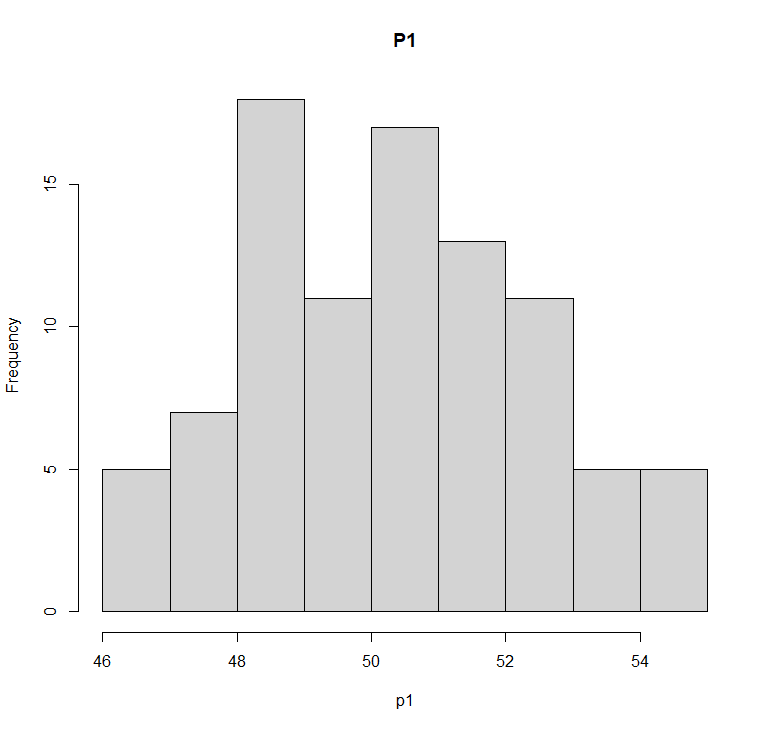
\includegraphics[width=0.9\textwidth]{figures/p1.png} % caminho do arquivo
    \caption{Histograma da simulação P1}
    \label{fig1}
\end{figure}

Já o conjunto p2, cujos valores foram obtidos a partir da função $p2 = a + b \cdot p1$, com $a = 5$ e $b = 3$, apresenta valores entre 143,8 e 169,4, indicando uma amplitude considerável. A média (155,8) e a mediana (155,6) são bastante próximas, assim como observado em p1, o que sugere simetria na distribuição. Os quartis mostram que 50\% das observações estão concentradas entre 150,7 (1º quartil) e 160,6 (3º quartil), evidenciando que a maior parte dos dados se encontra próxima do centro da distribuição. O desvio padrão é de aproximadamente 6,37, superior ao observado em p1, refletindo maior dispersão dos valores em torno da média. Ademais, o teste de Shapiro-Wilk (p-value = 0,1677) não rejeita a hipótese nula de normalidade (p > 0,05), o que confirma que os dados de p2 podem ser considerados normalmente distribuídos, resultado também evidenciado pela visualização do histograma (Figura~\ref{fig2}).

\begin{lstlisting}
# Para funcao: p2 = a + b*p1
a <- 5
b <- 3
p2 <- a + b*p1

summary(p2)
# Min. 1st Qu.  Median    Mean 3rd Qu.    Max. 
# 143.8   150.7   155.6   155.8   160.6   169.4

sd(p2)
# 6.373808

shapiro.test(p2)
# Shapiro-Wilk normality test
# data:  p2
# W = 0.97992, p-value = 0.1677

hist(p2, main="P2")
\end{lstlisting}

\begin{figure}[h] % [h] = here, [t] = top, [b] = bottom, [p] = página separada
    \centering
    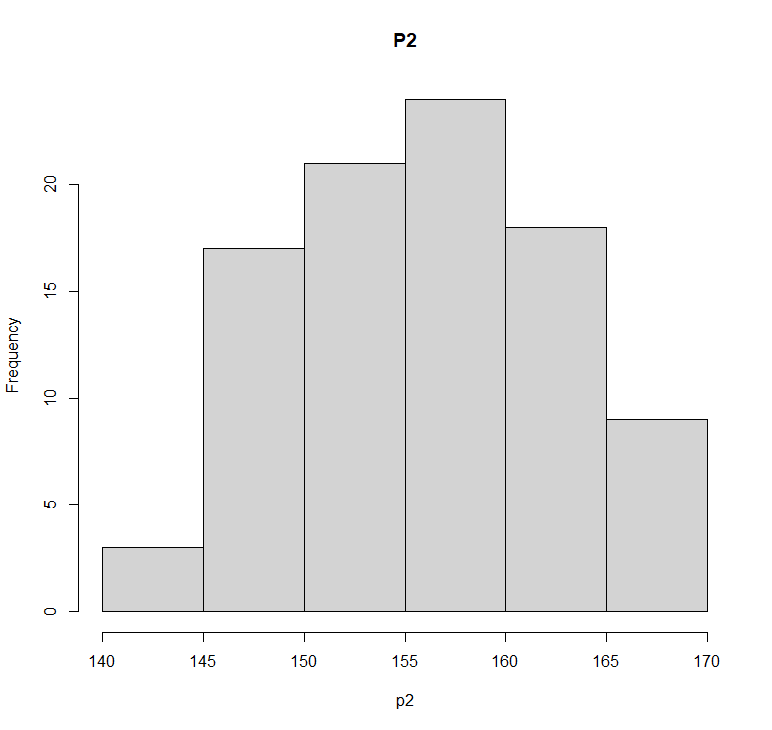
\includegraphics[width=0.9\textwidth]{figures/p2.png} % caminho do arquivo
    \caption{Histograma da simulação P2 = 5 + 3 x P1}
    \label{fig2}
\end{figure}

Como neste caso P1 e P2 satisfazem algumas condições:

\begin{itemize}
    \item Distribuição normal
    \item Média e desvio padrão conhecidos
    \item Dependência de P2 em P1
\end{itemize}

Podemos realizar um Teste t-Student com variáveis pareadas para verificar se as médias de P1 e P2 são estatisticamente diferentes. 

\begin{lstlisting}
t.test(p1, p2, paired=TRUE, conf.level = 0.95)

#Paired t-test
#data:  p1 and p2
#t = -238.23, df = 91, p-value < 2.2e-16
#alternative hypothesis: true mean difference is not equal to 0
#95 percent confidence interval:
#-106.4169 -104.6570
#sample estimates:
#mean difference -105.5369
\end{lstlisting}

Após realizar o teste t com confiança de 95\%, podemos afirmar que as médias de P1 e P2 são estatisticamente diferentes por dois motivos:
\begin{itemize}
    \item p-value < 0.05, o que implica que $H_0$ (Médias iguais) foi falseada
    \item O intervalo de confiança da diferença das médias $[-106.4169, -104.6570]$ não contém $0$
\end{itemize}

\section{Exercício 3}

\begin{lstlisting}
set.seed(153)

# Irei usar o mesmo desvio padrão para gerar os datasets para garantir homocedasticidade no exercício
# Gerar 4 datasets independentemente
# rnorm() para garantir distribuição normal em todos os conjuntos

var <- 5

# Gerar médias aleatórias entre [30,60] para serem as médias dos conjuntos
medias <- runif(4, min = 30, max = 60) 

n1_1 <- rnorm(35, mean = medias[1], sd = var)
n2_1 <- rnorm(35, mean = medias[2], sd = var)
n1_2 <- rnorm(57, mean = medias[3], sd = var)
n2_2 <- rnorm(57, mean = medias[4], sd = var)

summary(n1_1)
#Min. 1st Qu.  Median    Mean 3rd Qu.    Max. 
#48.50   56.03   59.43   59.12   61.58   69.00 
summary(n1_2)
#Min. 1st Qu.  Median    Mean 3rd Qu.    Max. 
#28.91   34.03   38.27   38.14   41.61   51.07 
summary(n2_1)
#Min. 1st Qu.  Median    Mean 3rd Qu.    Max. 
#36.16   41.33   43.63   44.61   48.14   53.12 
summary(n2_2)
#Min. 1st Qu.  Median    Mean 3rd Qu.    Max. 
#28.14   37.39   39.87   40.44   44.01   53.87

# Teste de normalidade dos conjuntos
shapiro.test(n1_1)
# W = 0.9859, p-value = 0.9242
shapiro.test(n1_2)
# W = 0.97733, p-value = 0.3593
shapiro.test(n2_1)
# W = 0.96533, p-value = 0.3282
shapiro.test(n2_2)
# W = 0.98261, p-value = 0.5827
# Todos os datasets são normais --> OK!
\end{lstlisting}

\begin{figure}[h]
    \centering
    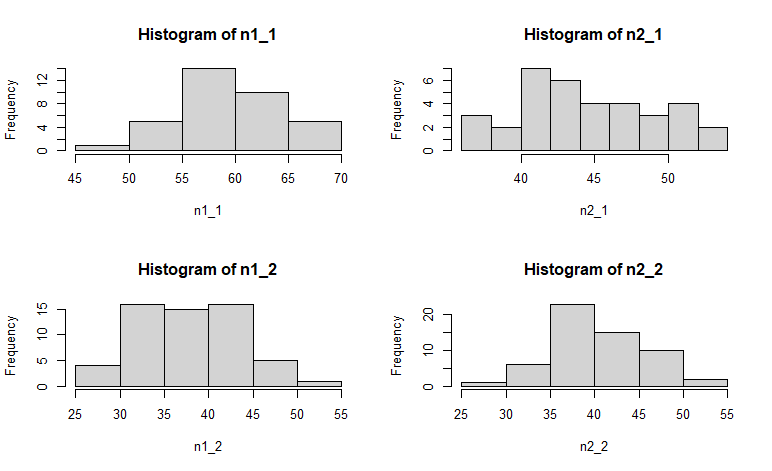
\includegraphics[width=0.9\textwidth]{figures/ex3.png} % caminho do arquivo
    \caption{Histograma das simulações}
    \label{fig3}
\end{figure}

\section{Exercício 4}

\end{document}